% !TEX root = sum1.tex
\section{Analyses of Model}

\subsection{Model for IVPU game}

A cooperative TU game $(V,c)$ is called an IVPU game if the characteristic function satisfies the following formulations.

\[
\begin{aligned}
c(s,P) = & {\min} \sum_{k\in V}\sum_{j\in O} {c_{kj} x_{kj}} + {P\sum_{k\in s} x_{k1}} \\
{s.t.}\quad & \sum_{j \in O} x_{kj}-y_k^s=0, \forall k \in V, \\
& \sum_{k\in V} x_{kj} \leq m,\forall j \in O,  \\
& x_{kj} \in \{0,1\} , \forall k \in V, \forall j \in O,\\
& y_k^s=1, k \in s, y_k^s=0, k \notin s.
\end{aligned}
\]

The first set of constraints indicate that only jobs in $s$ are included and are processed only once.
Notice that $ y_k^s=1, k \in s$, the constraints are equivalent to $\sum_{j \in O} x_{kj}-1=0, k \in s$.
The second set of constrains indicate that at most $m$
machines can be used, and they assure that no jobs are processed on the same machines at the same time.

Among these formulations, $P$ and $m$ denotes the price and maximum number of machines available, respectively. Note that $j$ represents the processing sequence on the machines, so when $j=1$, $\sum_{k\in s} x_{k1}$ indicates all machines used by coalition $s$, i.e., the optimal machine number.

To be consistent with the above definition of the grand coalition, let $V=\{1,2,\ldots,v\}$ be a set of $v$ players. The setup cost or price(We will use the term in the remainder of this article.) for each machine is $P$.

% For the convenience of expression, we set the processing times $t_i(i\in V)$ satisfy $t_1<t_2<\cdots<t_v$.

Then we need to define two functions, practical subsidy-price function (PSPF) and theoretical subsidy-price function (TSPF) denoted by $\omega(P)$ and $\hat{\omega}(P)$, respectively:
\[
  {\omega(P)}=\mathop{\min}_{\alpha}\{c(V,P)-\alpha(V): \alpha(s) \leq c(s,P)
 ,\forall s \in S, \alpha\in\mathbb{R}^{v}\},
\]
\[
  {\hat{\omega}(P)}=\mathop{\min}_{\alpha}\{c(V,P)-\alpha(V): \alpha(s) \leq c(s,P)
 ,\forall s \in S\setminus\{V\}, \alpha\in\mathbb{R}^{v}\}.
\]
PSPF has one more inequality $\alpha(V)\leq c(V,P)$ than TSPF, which ensures the minimum value of PSPF is 0, while TSPF can have a negative value. PSPF is our top priority because we think the value of subsidy is positive commonly. However, TSPF can also provide us with a theoretical perspective.

Then we need to define an interval $[P_L(i,V),P_H(i,V)]$ to denote the price range when the grand coalition $V$ uses $i$ machines to obtain the minimum cost for scheduling jobs. And the effective domain of pricing IVPU game for stabilization is $[0,P^*]$.
In other words, the price should have practical significance, that is, the negative price is beyond of our consideration in this situation. Thus, the minimum price for each machine is 0. Meanwhile, the maximum price for each machine will be infinity in theory, later we will show a more meaningful price instead of $P^*$ defined here.

Based on the above analysis, we know that $c(s,P) = \min_{i \in M} \{\sum_{k\in s}{C_k(i)}+ P\cdot i\}.$ Define a no-price characteristic function $c_0(s,i)$
related to the number of machines $i \in \{1,2,\ldots,v\}$ used by coalition $s.$ Meanwhile, $c_0(V,i)$ denotes the cost of using $i$ machines by the grand coalition and it is determined by $i$ when the processing time of every player in the grand coalition is known.
Therefore, the original characteristic function can be expressed in two parts like $c(s,P) = c_0(s,m^*) + P\cdot m^*$, where $m^*$ is the optimal number of machines used by coalition $s$.

We set the different intervals where the number of machines remain unchanged as $I_i$ respectively.
Assume that the optimal schedule is that the grand coalition uses $i$ machines, the price for each machine is $P^i$ which belongs to the interval $I_i$.
Then according to the definition of the characteristic function, we can obtain the following two inequalities:
\[
\begin{aligned}
&c_0 (V,i) + P^i i \leq c_0 (V,i-1) + P^i\cdot(i-1) \\
&c_0 (V,i) + P^i i \leq c_0 (V,i+1) + P^i\cdot(i+1).
\end{aligned}
\]
Consequently, we obtained the range of the price $P^i$ satisfies $c_0 (V,i) - c_0 (V,i+1) \leq P^i \leq c_0 (V,i-1) - c_0 (V,i)$.
That is to say, $P^i$ at least belongs to interval $[c_0 (V,i) - c_0 (V,i+1), c_0 (V,i-1) - c_0 (V,i)].$
We will continue to investigate the relationship between this interval and the above mentioned $I_i$.

% If we assume that the processing times satisfy $t_1 < t_2 < \ldots < t_v$, then $c_0(V,i) = \sum_{j=1}^{\lceil v/i \rceil} \sum_{h=1}^i j t_{v-ij-h+i+1}$, where $\lceil \cdot \rceil$ is the minimum integer larger than $\cdot$.

If we assume that the processing times satisfy $t_1 > t_2 > \ldots > t_v$, then $c_0(V,i) = \sum_{k=1}^{v} {\lceil k/i \rceil} t_{k}$, where $\lceil \cdot \rceil$ is the minimum integer larger than $\cdot$.

According to $c_0(V,i) = \sum_{k=1}^{v} {\lceil k/i \rceil} t_{k}$, it is easy to know that the multipliers of all the processing times $t_k, k \in V$ decrease correspondingly with the increase of the number of machines used.

Besides that, we can also prove that $\sum_{k=1}^{v} ({\lceil k/i \rceil} - {\lceil k/(i+1) \rceil}) t_k < \sum_{k=1}^{v} ({\lceil k/(i-1) \rceil} - {\lceil k/i \rceil}) t_k.$

Proof tips: Let $p_i(k)$ denote ${\lceil k/i \rceil}$, the $k$th multipliers of $t_k$. At first, $p_{i-1}(i)- p_i(i)=0 ~\text{or}~ 1$. Then the multiplier difference of $t_i$ is $p_{i-1}(i)- p_i(i)=1$, while $p_i(i) - p_{i+1}(i)=0$
Meanwhile, the multiplier difference of $t_{i+1}$ is $p_{i-1}(i+1)- p_i(i+1)=0$ and $p_i(i+1) - p_{i+1}(i+1)=1$. However, because of $t_{i} > t_{i+1}$, put the two numbers together we can get $(p_{i-1}(i)- p_i(i))t_i + (p_{i-1}(i+1)- p_i(i+1))t_{i+1} > (p_{i}(i)- p_{i+1}(i))t_i + (p_{i}(i+1)- p_i(i+1))t_{i+1}$.
The above relationship holds when the ordinal number $k$ satisfies $k = (l-1)i, l = \{2,3,\ldots,i\}$.
When $k > (i-1)i$, $p_{i-1}(k)- p_i(k) \geq p_{i}(k)- p_{i+1}(k)$. And when for other cases, it is easy to prove $p_{i-1}(k)- p_i(k) \geq p_{i}(k)- p_{i+1}(k)$.

So we have the following theorem:
\begin{thm}\label{thm1}
For the IVPU game, the no-price characteristic function $c_0(V,i)$ is monotone decreasing and concave with $i$, in other words, $c_0(V,i)$ satisfies the following inequalities:
\[
\begin{aligned}
& c_0(V,i)- c_0(V,i-1) < 0, i \in \{2,3,\ldots,v\}\\
& c_0 (V,i) - c_0 (V,i+1) < c_0 (V,i-1) - c_0 (V,i), i \in \{2,3,\ldots,v-1\}.
\end{aligned}
\]
\end{thm}

In the light of the Theorem \ref{thm1}, $c_0(V,i)- c_0(V,i-1) < 0$ ensures that the value of price is positive. Moreover, $c_0(V,i)$ is concave with $i$,  the interval will not be empty and $I_i = [c_0 (V,i) - c_0 (V,i+1), c_0 (V,i-1) - c_0 (V,i)], i \in \{2,3,\ldots,v-1\}.$ Define $I_1 = [c_0 (V,1) - c_0 (V,2), P^*]$ and $I_v = [0, c_0 (V,v-1) - c_0 (V,v)]$, until here, the effective domain $[0, P^*]$
is divided into $v$ non-overlapping sub-intervals $I_i, i\in V$.

\begin{remark}
  Denote the left and right extreme points of the interval $I_i$ as $P_L(i,V), P_H(i,V)$ respectively. It's easy to know that $P_L(i,V) = P_H(i+1,V)$.
\end{remark}

\begin{remark}
  Note that $P_L(i,V) = P_H(i+1,V)$, for the sake of brevity and readability, we use $P_{i+1}$ to substitute for $P_L(i,V)$ or $P_H(i+1,V)$ later on.
\end{remark}

\begin{remark}
  For ease of exposition, let $P_1 = P^*, P_L(v,V) = 0$ and $P_i = P_H(i,V) = P_L(i-1,V), i \in \{2,3,\ldots,v\}.$ Thus, the effective domain, $[0,P^*]$, is divided into $v$ non-overlapping sub-intervals by $P_i, \forall i \in \{2,3,\ldots,v\}$.
\end{remark}

\begin{remark}
  $P^*$ is the lowest price under which the grand cooperation of IVPU game is stable and it uses only one machine in the optimal scheduling decision, i.e.,
  $P^* \in (P_L(1,V), P_H(1,V)]$ and MSG$(V, c(\cdot, P^*))$ has non-empty core.
\end{remark}


\subsection{Properties of IVPU game}
Like the above, divide the characteristic function into two parts like $c(s,P) = c_0(s,m^*(s)) + P\cdot m^*(s), s \in S$.

As a common practice, we can obtain the dual of $\omega(P)$:
\begin{equation}\label{dual}
 {\omega^*(P)}=\mathop{\max}_{\rho} \{c_0(V)+m(V)P+\sum_{s\in S}-\rho_s[c_0(s,m^*(s)) + P\cdot m^*(s)]:
 \sum_{s\in S:k\in s}\rho_s=1,\forall k \in V,\rho_s\geq 0,\forall s \in S \}
\end{equation}

By deriving $\omega^*(P)$ with respect to $P$, we can obtain lemma \ref{lem1}.

\begin{lem}\label{lem1}
The sum of absolute values of slopes at both sides of $P_i$ is 1.
\end{lem}

Based on the above defined PSPF, we can establish Theorem \ref{thm2} below, showing the property of this function.

\begin{thm}\label{thm2}
$\omega(P)$ is piecewise linear, and convex in price P at each sub-interval $[P_{i+1},P_{i}], i \in \{1,2,\ldots,v-1\}$.
\end{thm}

In this situation, the size of interval $I_i$ can be calculated when $t_i,i \in \{1,2,\ldots,v\}$ is known. As shown previously, the extreme points of these intervals are recorded as $P_i$ respectively, which represents the price when the number of using machine changes from $i$ to $i-1$. Specially, $P_1$ denotes the right extreme point of the whole interval, which is the value of price when using one machine and subsidy equals zero.

Note that the costs of all the exponential coalitions can be easily calculated by the SPT rules, we have lemma \ref{lem2}.

\begin{lem}\label{lem2}
The breaking price, $P_i(2 \leq i \leq v)$, which is at the extreme points of the sub-intervals $I_i$ can be obtained by SPT rules in polynomial time.
\end{lem}

According to the above lemma \ref{lem2}, we can obtain all the extreme points of the sub-intervals $P_i, 2 \leq i \leq v$. When the price increase from $P_i^-$(little smaller than $P_i$) to $P_i^+$(little larger than $P_i$), the number of machines used by the grand coalition will decrease one.

\begin{thm}\label{thm3}
Boundary price $P^*$ or $P_1$ equals $\sum_{i=2}^v P_i$, and can be obtained in polynomial time.
\end{thm}

With theorem \ref{thm3}, we obtain all the breakpoints during the whole price interval $[0,P^*]$. Then we'll focus on the specific property of subsidy.

\begin{thm}\label{thm4}
$\omega(P)$ can be bounded by zero when the number of machines used by the grand coalition $V$ is larger than $\frac{v}{2}$.
\end{thm}

In other words, when the number of machines used is larger than half of players, the grand coalition doesnot need any subsidy from the externality.

Define a new game, that is Single Machine Scheduling Game(SMSG)
\[
\begin{aligned}
c(s,P,'m='1) = & {\min} \sum_{k\in V}\sum_{j\in O} {c_{kj} x_{kj} + P} \\
{s.t.}\quad & \sum_{j \in O} x_{kj}-y_k^s=0, \forall k \in V, \\
& \sum_{k\in V} x_{kj} \leq 1, \forall j \in O,  \\
& x_{kj} \in \{0,1\} , \forall k \in V, \forall j \in O,\\
& y_k^s=1, k \in s, y_k^s=0, k \notin s.
\end{aligned}
\]

\begin{thm}\label{thm5}
For SMSG(or, MSG with only one machine), given $P \in [P_2, P^*]$ (or, $[P_2,P_1]$),
the slope range of each segments in the interval for function $\omega(P)$ is within $\left(-1, -\frac{1}{n-1} \right]$, and the number of breakpoints in the same interval for function $\omega(P)$ is within $O(v^2)$.
\end{thm}

Until here, we described the main property of the whole figure.
And a diagram of the number of machines used and subsidy on price with essential features is showed below.

\begin{figure}[h]%%图
	\centering  %插入的图片居中表示
	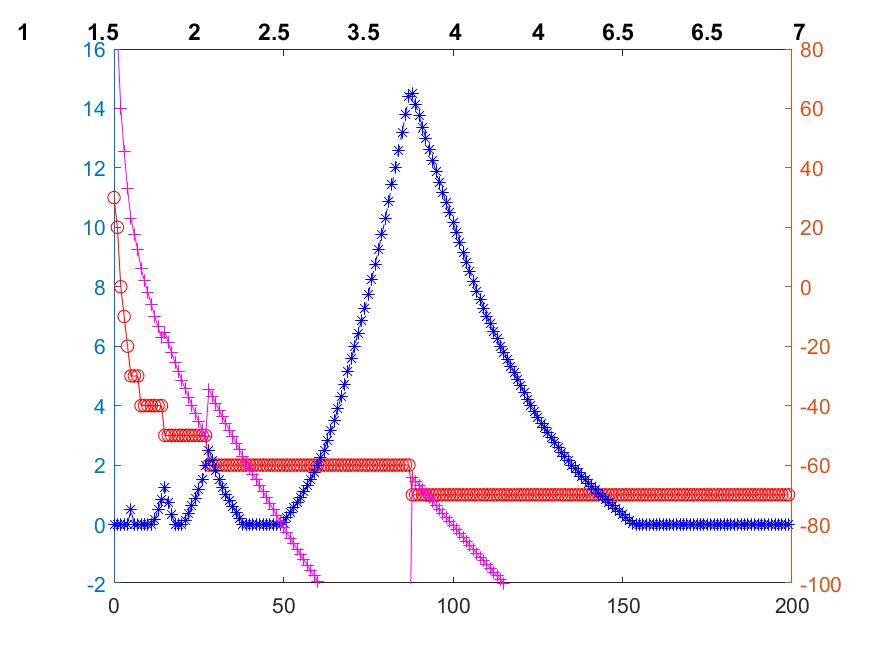
\includegraphics[width=0.8\linewidth]{Figures/Image30}  %插入的图,包括JPG,PNG,PDF,EPS等,放在源文件目录下
	\caption{The number of machines and subsidy on setup cost.}  %图片的名称
	\label{fig:Image11}   %标签,用作引用
\end{figure}

% 这里把图画一下,然后进行比较

\begin{remark}
  When the number of available machines $m$ is larger than $v$, the image is complete, just like the above shown. However, when the number of available machines $m$ is less than $v$, the image will be truncated, which means the corresponding part of the price less than $P_{m+1}$ should be removed from the figure. While the properties of the rest part will still hold.
\end{remark}

The processing times of all jobs with the arrangement from small to large are listed on the top of this figure.
The red and blue lines stand for the machine number and subsidy, respectively.
The horizontal ordinate represents the price.
The left ordinate represents the number of machine used, while the right represents the value of subsidy.

Compared with the traditional characteristic function $c(s)$, characteristic function defined in the IVPU game has another parameter, the number of machines used by coalition $m(s)$, whose exponential numbers of $m(s)$ bring more difficulties to the solution.
In order to address this problem, we establish the Theorem \ref{thm5}.

\begin{thm}\label{thm7}
  Define that
  \[
    {\omega_1(P)}=\mathop{\min}_{\alpha}\{c(V,P)-\alpha(V): \alpha(s)\leq c(s,P,1), \forall s \in S, \alpha\in\mathbb{R}^{v}\},
  \]
then the original problem $\omega(P)$ is equivalent to $\omega_1(P)$.
\end{thm}

As the coalitional stability constraints showed above, the exponential inequality constraints are so tricky that we must figure out a method to eliminate redundant constraints to obtain the optimal results.

With the Theorem 5, which will save us from the trouble of solving $c(s, P)$ and speed up the solution, we can use the cutting plane method to eliminate the redundant inequalitie, then  any value of $\omega_1(P)$ can be polynomially solvable when given $P$.
